%%%%%%%%%%%%%%%%%%%%%%%%%%%%%%%%%%%%%%%%%%%%%%%%%%%%%%%%%%%%
%%%%%%%%%%%%%%%%%%%%%%%%%%%%%%%%%%%%%%%%%%%%%%%%%%%%%%%%%%%%
%%%%%%%%%%%%%%%%%%%%%%%%%%%%%%%%%%%%%%%%%%%%%%%%%%%%%%%%%%%%
\section{Unconstrained Conforming Finite Elements}\label{Sec:EllipticProblems}
\subsection{Introduction}
%%%%%%%%%%%%%%%%%%%%%%%%%%%%%%%%%%%%%%%%%%%%%%%%%%%%%%%%%%%%
%%%%%%%%%%%%%%%%%%%%%%%%%%%%%%%%%%%%%%%%%%%%%%%%%%%%%%%%%%%%
%%%%%%%%%%%%%%%%%%%%%%%%%%%%%%%%%%%%%%%%%%%%%%%%%%%%%%%%%%%%

%\subsection{PDELab Aims and Features}

\begin{frame}
\frametitle<presentation>{DUNE PDELab Features}
\begin{itemize}
\item \textbf{Substantially reduce time to implement
discretizations and solvers for systems of PDEs based on DUNE.}
%\item Simple things should be simple --- but still be efficient!
\item \textbf{Discrete function spaces}
\begin{itemize}
\item Map element-wise to global degrees of freedom.
\item Seperate DOF mapping and coefficient vectors.
\item General approach to constraints.
\item Nested product spaces for systems of PDEs.
\item Handle communication on distributed grids.
\end{itemize}
\item \textbf{Generic Finite Element Assembly}
\begin{itemize}
\item Handle element and face integrals.
\item Residual and matrix assembly.
\item Linear and nonlinear, stationary and transient problems.
\end{itemize}
\item \textbf{Solvers}
\begin{itemize}
\item Exploitation of blocking and ordering in linear solvers.
\item Nonlinear solver (Newton, Picard, \ldots).
\item Single step time-stepping schemes (explicit, implicit).
\end{itemize}
\item Exchangeable linear algebra backend
\item Still have to write C++ code, full control on element level.
%\item User only involved with ``local'' view on (reference) element.
\end{itemize}
\end{frame}

\begin{frame}
\frametitle<presentation>{Coding Effort}
\begin{center}
\small\begin{tabular}{|p{0.5\textwidth}|p{0.3\textwidth}|r|}
\hline
Problem & Scheme & LOC \\
\hline
\hline
$\nabla\cdot\{v u - K\nabla u\}=f$ & $P_k, Q_k$ & 643 \\
 & DG & 1034 \\
\hline
$-\nabla\cdot\{K\nabla u\}=f$ & CCFV & 223 \\
 & RT$_0$ & 289 \\
 & Mimetic & 278 \\
\hline
Two-phase flow in porous media & $p_l, p_c$, CCFV & 700 \\
& $p_l, p_c$, DG & 931 \\
& CCFV, 2c & 986 \\
\hline
Navier-Stokes & $P_2/P_1$, $Q_2/Q_1$ & 539 \\
           & DG & 1122 \\
\hline
Linear acoustics & DG & 700 \\
\hline
Maxwell in time domain & DG & 857 \\
 & Nedelec & 488 \\
\hline
\end{tabular}
\end{center}
This does \textbf{not} include finite element spaces and problem setup.
\end{frame}

\begin{frame}
\frametitle<presentation>{DUNE Module Architecture}
Major DUNE modules are:
\begin{center}
\mode<presentation>{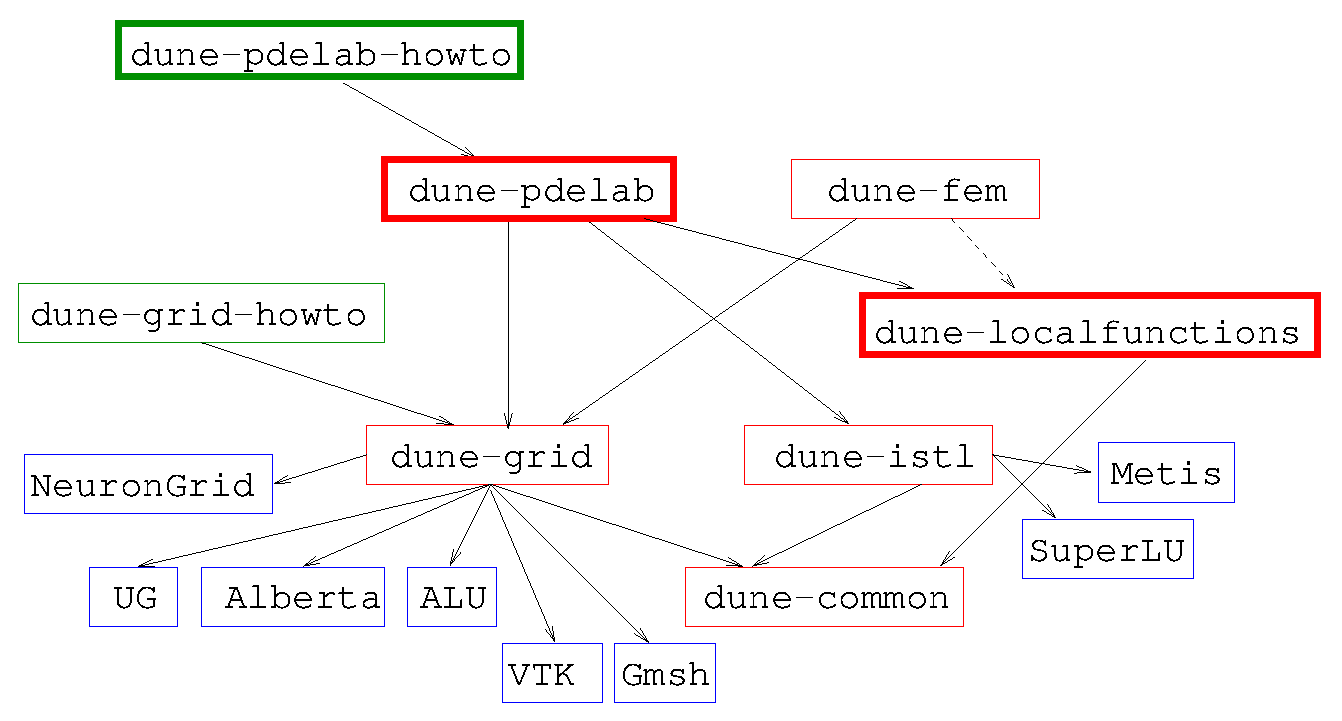
\includegraphics[width=1.0\textwidth]{./EPS/modules}}
\mode<article>{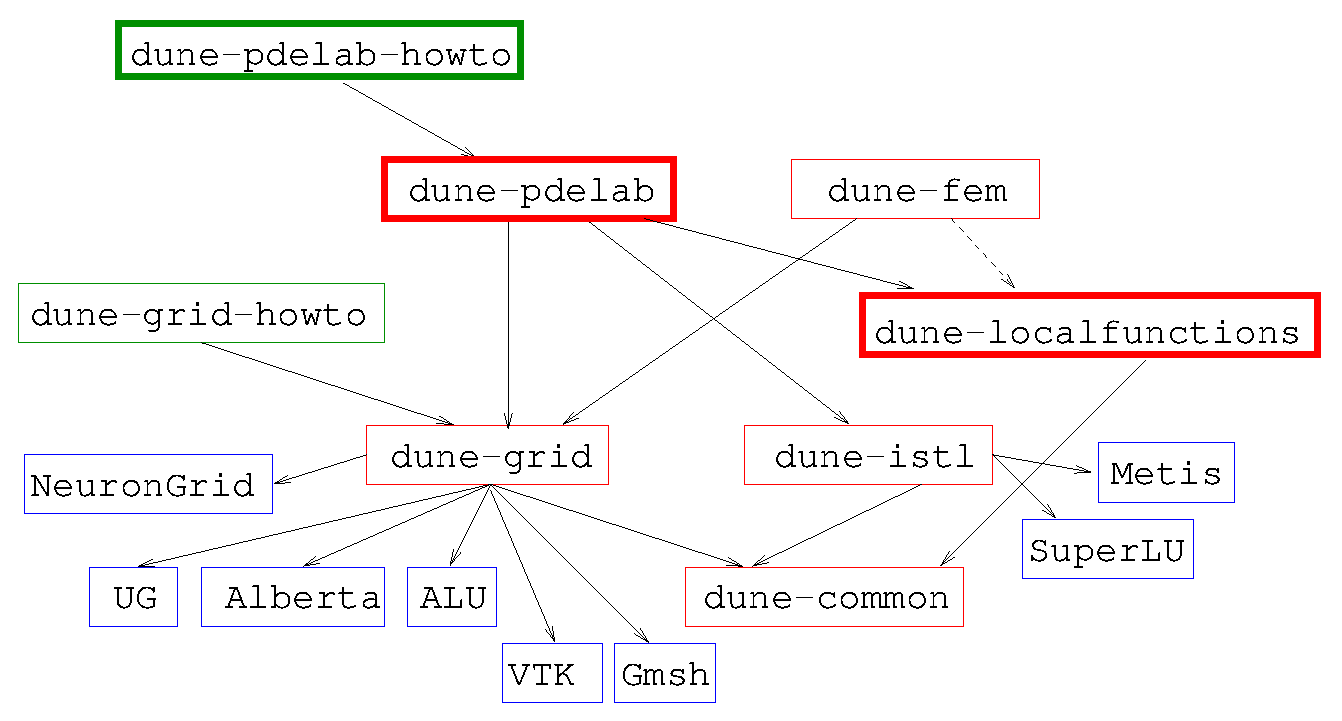
\includegraphics[width=0.7\textwidth]{./EPS/modules}}
\end{center}
\end{frame}

\begin{frame}
\frametitle<presentation>{Required Modules}
To work through the examples the following DUNE modules are required:
\begin{itemize}
\item \lstinline{dune-common},
\item \lstinline{dune-geometry},
\item \lstinline{dune-grid},
\item \lstinline{dune-istl},
\item \lstinline{dune-localfunctions},
\item \lstinline{dune-typetree},
\item \lstinline{dune-pdelab},
\item \lstinline{dune-pdelab-howto},
\end{itemize}

In addition, at least one of the grid managers UG, ALU or Alberta is
required to do the examples on simplex grids.
\end{frame}



\subsection<article>{How to Read this Manual}

The main idea of this howto is to introduce the concepts by working
through a set of increasingly complex examples. We will start by
solving stationary elliptic problems first without and then with constrained spaces
(Dirichlet boundary conditions). After some excursion to linear algebra backends and
working with CAD models instationary problems and systems will be treated.

\cleardoublepage
